\documentclass[11pt,a4paper]{article}
\usepackage[utf8]{inputenc}
\usepackage{algorithm}
\usepackage{algorithmic}
\usepackage{amsmath}
\usepackage{amsfonts}
\usepackage{amssymb}
\usepackage{amsthm}
\usepackage{cite}
\usepackage{graphicx}
\usepackage{listings}



\newtheorem{theorem}{Theorem}[section]
\newtheorem{corollary}{Corollary}[theorem]
\newtheorem{lemma}[theorem]{Lemma}
 
\author{Duong Thanh Dat (A0119656), Ramon Bespinyowong (A0088687)}
\title{Mini-Project 3: Airport Scheduling}



\begin{document}

\maketitle

%\begin{abstract}
%\end{abstract}


\section{Overview}
\label{sec:over}

\subsection{Introduction}
\label{subesc:over-intr}
Gate scheduling for flights is a key operation at airports and is an important problem. Due to globalization, more people are travelling around the world and hence more air transportations are used. Each aircraft is assigned to a terminal, called gates. To handle increasing in traffic volume, we have to assign planes to gates efficiently so that the airport can take more aircraft or more passengers. \par
In this assignment, we study the airport scheduling problem. Given schedules of planes landing and taking-off at the airport, we are required to assign each flight to a gate based on the schedules. The number of required gates must be minimum. \par
There are four problems of airport scheduling problems in this work. The first problem assumes that each plane takes a point of time to land and take off at the airport. The second problem assumes that each plane task has a starting time and an ending time. The third problem studies about the effect of delay in the algorithm used in the first two problems. Finally, the last problem assumes that reallocating planes to new gates is so expensive that we have to design such an algorithm that minimize the reassignments. In other words, we must create such an initial assignment that leaves many buffer time in the schedule as much as possible.  \par
In this work, we purpose algorithms to solve all the problems in Subsections~\ref{subsec:algo-prob1}, ~\ref{subsec:algo-prob2}, ~\ref{subsec:algo-prob3}, and ~\ref{subsec:algo-prob4} respectively. \par
The rest of the work is organized as follows: In the rest of Section~\ref{sec:over} we provide the background and an overview of the related work. Section~\ref{sec:algo} presents algorithms to all four problems of airport scheduling problems. In Section~\ref{sec:expe} we present a thorough experimental study of our algorithms. Finally, Section~\ref{sec:conc} concludes our work and states future plans. \par

\subsection{Preliminaries and Related Work}
\label{subsec:over-prel}
Let $G=\{g_1, ..., g_{|G|}\}$ be a set of gates and $A=\{a_1, ..., a_{|A|}\}$ be a set of planes. Each plane, $a_i$, needs to use any gate from $s_i$ to $f_i$. We need to find optimal solution which uses the fewest number of gates and all the planes have an allocation to any gate in the airport from $s_i$ to $f_i$. In addition, each gate can only take one plane for a particular time. \par
In this Subsection, we are going to look at similar problems to airport scheduling problems.

\subsubsection{Interval Scheduling}
Interval scheduling problems are also known as \textit{fixed job scheduling} or \textit{k-track assignment} problems~\cite{Lenstra2006}. They are different from other scheduling problems in such a way that the starting time of each job is fixed. \par
The formal problem description is given as follows: \textit{n} interval \textit{jobs}, $A = \{a_1, ..., a_{|A|}\}$, in the form [$s_j$, $f_j$) with $0 \leq s_j < f_j$ for $j = 1, ..., n$. These jobs must be processed uninterruptedly. There are \textit{machines}, $M=\{m_1, ..., m_{|M|}\}$. each of which can process at most one job at a time and is always available from $t \in [0, \infty)$. A \textit{schedule} is an assignment of some of the jobs to the machines. \par
We can view airport scheduling problems as interval scheduling problems. Let each gate be a machine and each plane be a job. The time needed at the gate is the process time of each job. \par
There exists several algorithms for solving this algorithm. The lower bound for the number of machines required for processing all the jobs is equal to the largest size of the a subset of jobs that pairwise overlap. Dilworth's chain decomposition is used to show that this lower bound suffices to process all jobs~\cite{Lenstra2006}. Ford and Fulkerson~\cite{FordL.r.1962} can solve this in $O(n^2)$ by using \textit{staircase rule} based on Dilworth's theorem. Alternative procedures are purposed by Hashimoto and Stevens~\cite{hashimoto1971wire} and Gertsbakh and Stern~\cite{gertsbakh1978minimal}. An $O(nlogn)$ procedure is proposed by Gupta et al~\cite{gupta1979optimal}, which will be further explained in Subsection~\ref{subsec:algo-prob2}. There even exists an $O(log n)$ algorithm with $O(n^2/log n)$ processors by Dekel and Sahni~\cite{dekel1983parallel}. \par
%There is a variant of interval scheduling problems called \textit{Interval Scheduling Maximization} which is to find a largest set of non-overlapping jobs to fit one machine. We can get optimal solution by greedy algorithm shown in Algorithm~\ref{algo:greedy}. This algorithm firstly sorts all the jobs based on earliest end time. It is interesting that sorting by the lengths of intervals, by the number of conflicts, or by the starting times does not give optimal solution. Then, the algorithm greedily takes the job with the earliest end time and remove every other jobs that has a conflict with this job. The algorithm continues picking the next earliest jobs until all the jobs are exhausted. The time complexity of this algorithm is $O(|J| log |J|)$ from a sorting algorithm used in the algorithm. \par
%
%\begin{algorithm}
%\caption{Greedy Algorithm for Scheduling Problms}
%\label{algo:greedy}
%\begin{algorithmic}
%	\STATE Sort jobs by ending time
%	\STATE $S \gets \emptyset$
%	\WHILE {$A \neq \emptyset$}
%		\STATE $a_i \gets $ the job with the earliest end time in $A$.
%		\STATE $S \gets S \cup \{a_i\}$
%		\STATE $A \gets A - \{a_j | [s_j, f_j) \cap [s_i, f_i) \neq \emptyset\}$
%	\ENDWHILE
%	\RETURN $A$
%\end{algorithmic}
%\end{algorithm}
%
%In Subsection~\ref{subsec:algo-prob2}, where Problem 2 is discussed, this algorithm will be applied on multiple machines. In other words, some changes will be made to this algorithm to make it compatible to the airport scheduling problems which have more than one gate.

\section{Algorithms and Theory}
\label{sec:algo}

\subsection{Problem 1}
\label{subsec:algo-prob1}
We are asked to explore the flight dataset and make some observations. The result can be found in Subsection~\ref{subsec:expo-data}. \par
Next, the first problem asks us to find an algorithm for the simplified version of airport scheduling problems where the starting time and the ending time of each plane is the same. Here, we propose Algorithm~\ref{algo:p1}. \par

\begin{algorithm}
\caption{Simple Airport Scheduling} \label{algo:p1}
\begin{algorithmic}
\STATE $G \gets \emptyset$
\FORALL{$a_i$ in A}
	\STATE $g \gets $ an available gate in G at time, $s_i$
	\IF{There is no such $g$}
		\STATE $g \gets $ a new gate
		\STATE $G \gets G \cup \{g\}$
	\ENDIF
	\STATE $g$ is allocated $a_i$
\ENDFOR
\end{algorithmic}
\end{algorithm}

This algorithm can solve airport scheduling problems because all the planes are assigned to at least a gate. Time complexity is $O(|A|)$ if all procedures such as finding an available gate can be done in $O(1)$. We are going to prove that this algorithm gives the smallest number of required gates. \par
\begin{theorem}
Algorithm~\ref{algo:p1} uses $k$ gates where $k$ is the maximum number of overlapping starting time of all the planes.
\end{theorem}
\begin{proof}
Assume, for the sake of contradiction, that Algorithm~\ref{algo:p1} uses more than $k$ gates. Therefore, there must be at least $k+1$ gates. Let $a_i$ be the first plane assigned to the $(k+1)$\textsuperscript{th} gate. Therefore, before $a_i$ is selected, there are $k$ gates. In order for a new gate to be created, there must not be any available gates in $G$ at time $s_i$. Since a new gate is created, all $k$ gates must be occupied by some planes. Therefore, there are $k+1$ planes coming to the airport at $s_i$, which contradicts the definition of $k$.
\end{proof}
Next, we are going to show that this algorithm gives the optimal number of gates.
\begin{lemma}
The lower bound of the number of gates is $k$.
\end{lemma}
\begin{proof}
This can be proven by Dilworth's theorem as mentioned in Subsection~\ref{subsec:over-prel}. But we will use a simpler proof here. Suppose that the number of gates can be less than $k$. Therefore, the number of gates is less than or equal to $k-1$. Assume, for the sake of a contradiction, that $k-1$ is the possible number of gates. Let $t$ be when there are $k$ overlapping taking-off times of planes. Suppose that all $k-1$ planes have been assigned to gates. The $k^{th}$ plane cannot be scheduled to any gate as all the gates are occupied by earlier $k-1$ planes. Hence, $k-1$ is not a possible solution. We can use this prove for any number of planes less than $k$. Therefore, the number of gates must be greater than or equal to $k$.
%According to Dilworth's theorem, the maximum number of elements in any antichain, a set of elements no two of which are comparable to each other, equals to the minimum number of chains in any partition of the set into chains. In this case, the maximum number of overlapping starting time of all the planes is the maximum number of elements in any antichain. Therefore, the minimum number of chains which is the number of required gates is equal to $k$.
\end{proof}

\begin{theorem}
Algorithm~\ref{algo:p1} gives the optimal solution.
\end{theorem}
\begin{proof}
Let $OPT$ be the smallest number of gates required and $ANS$ be the number of gates used in Algorithm~\ref{algo:p1}. According to the previous lemma, $OPT \geq k$. But, $k$ is the number of required gates from this algorithm. Hence, $OPT \geq ANS$. In addition, $ANS \geq OPT$ because there cannot be any better solutions than the optimal solution. Hence, $ANS = OPT$.
\end{proof}


\subsection{Problem 2}
\label{subsec:algo-prob2}
In this problem, we are given an amount of time we need at a gate for a plane to take-off and arrive at the airport. Each plane needs 90 minutes before the scheduled and 30 minutes after the scheduled take-off time at a gate. Therefore, for a plane, $a_i$, taking off at time $t_i$, we can use interval $[s_i, f_i) = [t_i-90, t_i+30)$ to represent the time the plane needs at a gate. \par
We propose greedy algorithm, Algorithm~\ref{algo:p2}. The algorithm firstly sorts all the planes by starting time. Then, the algorithm iterates over all the planes. The algorithm assigns a plane to an empty gate. However, if there does not exist any empty gate at the start time of the plane, the algorithm will create a new gate and assign the gate to the plane. \par

\begin{algorithm}
\caption{Greedy Algorithm for Airport Scheduling}\label{algo:p2}
\begin{algorithmic}
\STATE \textbf{Sort} $A$ by starting time
\STATE $G \gets \emptyset$
\FORALL{$a_i$ in A}
	\STATE $g \gets $ a gate, $g \in G$, vacant at $s_i$.
	\IF{There is no such $g$}
		\STATE $g \gets$ a new gate \label{algo:p2:newGate}
		\STATE $G \gets G \cup \{g\}$
	\ENDIF
	\STATE schedule $a_i$ to $g$ \label{algo:p2:schedule}
\ENDFOR
\end{algorithmic}
\end{algorithm}

Next, we show that this algorithm works correctly. All the planes have a gate for taking off. In addition, all the gates can have at most 1 plane at a particular time. In addition, we also show that Algorithm~\ref{algo:p2} is optimal. In other words, the number of gates is minimum.\par

\begin{theorem}
All the planes have a gate, $g$, for taking-off. At a particular time, $t$, a gate has at most 1 plane.
\end{theorem}
\begin{proof}
Line~\ref{algo:p2:schedule} of Algorithm~\ref{algo:p2} schedules every plane. Therefore, all the planes must have a gate during its taking-off time. \par
Next, we show that a gate has at most 1 plane at a particular point of time, $t$. Assume, for the sake of contradiction, that there exists such a gate, $g$, that there are more than a plane at $t$. Therefore, there must be at least two planes at time $t$ at $g$ after executing this algorithm. Let $a_i$ and $a_j$ be the first plane and the second plane assigned to $g$. When $a_j$ is scheduled to $g$, $g$ cannot be a new gate from Line~\ref{algo:p2:newGate} because this gate was already scheduled to $a_i$. Therefore, the if-condition must be wrong. Hence, $g$ is a gate that is vacant at $s_j$. Because of the greedy property, $s_i < s_j$. In addition, $f_i \leq s_j$ because $g$ is empty at $s_j$. Hence, these two planes' intervals do not overlap and they cannot be assigned to any gate at any time. \par
Therefore, this algorithm can schedule aircraft to gates correctly.
\end{proof}

Let $OPT$ and $ANS$ be the optimal number of gates and the number of gates from the algorithm respectively. \par

\begin{lemma}
$ANS \geq OPT$ 
\end{lemma}
\begin{proof}
No other possible solutions have the fewer number of gates than the optimal solution.
\end{proof}

\begin{lemma}
Let the maximum number of overlapping intervals be $k$. $k$ is the lower bound of this problem.
\end{lemma}
\begin{proof}
Assume, for the sake of contradiction, the possible number of gates is less than $k$. Let time $t$ be when the maximum number of overlapping intervals occurs. Therefore, there must be a plane that is not scheduled to any gate as all the other gates are occupied. Hence, this solution is not possible.
\end{proof}

\begin{lemma}
$ANS = k$
\end{lemma}
\begin{proof}
Assume, for the sake of contradiction, $ANS \neq k$. Therefore, $ANS < k$ or $ANS > k$. \par
\underline{case 1} $ANS < k$: This is impossible because $k$ is the lower bound and $ANS$ is a valid solution. Therefore, $ANS \geq k$. \par
\underline{case 2} $ANS > k$: Therefore, $ANS$ must be at least $k+1$. Let $a_i$ be a plane that is firstly assigned to $g_{k+1}$. Therefore, there is no empty gate in $G$ at $s_i$ when $|G| = k$. Therefore, all $k$ gates have planes. Hence, there are $k+1$ planes overlapping at $s_i$. This is a contradiction because $k$ is the maximum number of overlapping intervals. \par
Therefore, $ANS = k$
\end{proof}

\begin{theorem}
The number of gates from Algorithm~\ref{algo:p2} is equal to the optimal number of gates.
\end{theorem}
\begin{proof}
$k$ is the lower bound and is equal to $ANS$. Therefore, $OPT \geq k = ANS$. We can conclude that $OPT = ANS$ because $OPT \geq ANS$ and $ANS \geq OPT$.
\end{proof}

After showing that the greedy algorithm is optimal, we use this algorithm on real dataset and the result is shown in Subsection~\ref{subsec:expo-resu}. \par

\subsubsection{Doubling the Number of Gates}
We also introduce one more interesting problem here: \textbf{do we need to double the number of gates to support twice as many flights?} It depends on how we increase the number of flights. Suppose that at first intervals $[0, t_1)$ and $[t_1, t_2)$ have the maximum number of overlapping plane taking-off intervals $2x$ and $x$ respectively. Therefore, we need $2x$ gates. Now we double the flights by adding $x$ and $2x$ plane intervals to time $[0, t_1)$ and $[t_1, t_2)$ respectively. Therefore, we will need at most $3x$ gates and $3x$ is not as many as twice of $2x$. \par
In addition, it is also possible that we need more than twice of the number of current gates. Again, assume that at first there are at most $x$ overlapping schedules in both intervals $[0, t_1)$ and $[t_1, t_2)$. We double the number of flights by adding $2x$ planes to the first interval and make those $2x$ planes cover time $t_a$, where there were previously $x$ overlapping intervals. Therefore, now there are $3x$ overlapping intervals. Hence, we need $3x$ gates which is more than two times of the previous number of gates required.

\subsection{Problem 3}
\label{subsec:algo-prob3}
Most of the time, the flights are delayed and rescheduling is required. Sometimes, we need overflow gates if there are not enough gates. Overflow gates happen when we have already scheduled a plane to the gate; however, there is a delay from the previous flight. Therefore, the gate must be occupied for the previous flight longer than expected. Hence, the incoming flight has to go to an overflow gate. In this section, we develop an algorithm for solving this problem. Although the optimal solution requires rescheduling all the future flights from the point of gate collision as shown in Algorithm~\ref{algo:p3-opt}. We are not interested in that solution as the time complexity is large and it is costly to reschedule every other flight. Let each gate interval has two kinds of intervals: the scheduled interval, $[s_i, t_i)$, and the actual interval, $[s_i*, t_i*)$. We propose Algorithm~\ref{algo:p3} to solve the gate collision. In addition, we propose another algorithm that takes all the collided gate intervals and run Algorithm~\ref{algo:p2} on those collided gate intervals to find the number of total gates.\par

\begin{algorithm}
\caption{optimal overflow gate scheduling}
\label{algo:p3-opt}
\begin{algorithmic}
\STATE \textbf{Given} $G$, a set of gate with scheduled flights.
\STATE \textbf{Given} $C$, a set of intervals of gate collision.
\STATE $A \gets \{[s_i*, t_i*) | i \in C\} \cup \{[s_i, t_i) | i \in G-C\}$
\STATE \textbf{sort} $A$ by its starting time.
\STATE $G \gets \emptyset$
\FORALL{$a_i$ in A}
	\STATE $g \gets $ a gate, $g \in G$, vacant at $s_i$.
	\IF{There is no such $g$}
		\STATE $g \gets$ a new gate \label{algo:p2:newGate}
		\STATE $G \gets G \cup \{g\}$
	\ENDIF
	\STATE schedule $a_i$ to $g$ \label{algo:p2:schedule}
\ENDFOR
\end{algorithmic}
\end{algorithm}

\begin{algorithm}
\caption{overflow gate scheduling}\label{algo:p3}
\begin{algorithmic}
\STATE \textbf{Given} $G$, a set of gate with scheduled flights.
\STATE \textbf{Given} $C$, a set of intervals of gate collision.
\STATE remove $C$ from $G$.
\STATE $O \gets \emptyset$
\STATE \textbf{Sort} $C$ by starting time
\FORALL{$[s_i*, t_i*)$ in $C$}
	\STATE $g \gets $ a gate, $g \in G$, vacant at $[s_i*, t_i*)$
	\IF{There is no such $g$}
		\STATE $o \gets $ a gate $\in O$, vacant at $[s_i*, t_i*)$
		\IF{There is no such $o$}
			\STATE $o \gets$ a new gate
			\STATE $O \gets O \cup \{o\}$
		\ENDIF
		\STATE $g \gets o$
	\ENDIF
	\STATE schedule $[s_i*, t_i*)$ to $g$
\ENDFOR
\RETURN a set of overflow gate, $O$
\end{algorithmic}
\end{algorithm}


\subsection{Problem 4}
\label{subsec:algo-prob4}

\section{Experiments}
\label{sec:expe}

\subsection{Methodology}
\label{subsec:expo-meth}
\subsubsection{Data Set Analysis}
\label{subsec:expo-data}
\paragraph{Dataset selection}
We use US flight dataset from Research of Innovative Technology Administration Bureau of Transportation Statistics (RITA)~\cite{rita}. This dataset contains: time period, airline information, origin, destination, departure performance, arrival performance, cancellations and diversions, flight summaries, cause of delay. We are only interested in departure performance and arrival performance which are related to gate scheduling. We decide to use the information in January because there is new year holiday at the beginning of the month and it is interesting to see the effect of holiday on flights. In addition, we decide to choose the most busy airport. We define the most busy airport as the airport with highest number of outgoing and incoming flights. In this section, certain analyses on traffic and on delay are done. The SQL codes used for analysis can be found in Appendix.

\paragraph{Traffic analysis}
In January, Dallas/Fort Worth International Airport (DFW) of which id is 11298 is the airport with the highest traffic as shown in Table~\ref{fig:airport-flight-out} and Table~\ref{fig:airport-flight-in}.\par

\begin{table}
\caption{Airports with top 5 highest number of outgoing flights}
\centering
\begin{tabular}{| c | c |}
\hline
airportId & total flights \\
\hline
11298&23488 \\
13930&21497 \\
12892&18481 \\
11292&17977 \\
12266&14581 \\
\hline
\end{tabular}
\label{fig:airport-flight-out}
\end{table}

\begin{table}
\caption{Airports with top 5 highest number of incoming flights}
\centering
\begin{tabular}{| c | c |}
\hline
airportId & total flights \\
\hline
10397&30784 \\
11298&23482 \\
13930&21529 \\
12892&18474 \\
11292&17955 \\
\hline
\end{tabular}
\label{fig:airport-flight-in}
\end{table}

In addition, the top three dates with the highest number of flight are 3rd, 2nd, and 6th January. This is reasonable because they are at the end of the new year holiday where people need to go back home and come back from their vacation.

\paragraph{Delay Analysis}
Regarding delay, there are 255198 flights with delay while there are only 471949 flights. Therefore, more than half of the flights are delayed. Hence, airport scheduling should consider the delay effect as well. This is what we model in Problem 3. \par
Based on outgoing flights from DFW where there is the highest traffic, the top three days with highest delay are 6th, 2nd, and 9th January. This is quite reasonable as people travel a lot at the beginning of the month due to New Year holiday. In addition, the first two days also has rankings amongst the top three days with the highest number of total flights in DFW as shown in Table~\ref{table:airport-dfw-delay}.

\begin{table}
\caption{Days with highest number of flights and highest average delays in DFW}
\centering
\begin{tabular}{| c | c | c | c |}
\hline
Order & Most traffic & Highest average delay & Average delay \\
\hline
1 & 2 January 2014 & 6 January 2014 & 33.62\\
2 & 3 January 2014 & 2 January 2014 & 23.96\\
3 & 6 January 2014 & 9 January 2014 & 21.63\\
4 & 31 January 2014 & 5 January 2014 & 21.60\\
5 & 17 January 2014 & 7 January 2014 & 19.44\\
\hline
\end{tabular}
\label{table:airport-dfw-delay}
\end{table}

%Knowing that the most traffic happens on these five days, we run our scheduling algorithm assuming that there is no delay to find out how many gates we need. The result can be found in Section~\ref{subsec:expo-resu}. \par 
%In addition, we are also interested in the effect of delays to the number of gates. We decide to run our algorithm on 2nd of January to see how well the algorithm does when there are a lot of delays. In addition, we also decide to run an experiment on 15th January which have the lowest average delay, 4.21 minutes.

\subsection{Main Results}
\label{subsec:expo-resu}
\subsubsection{The number of Gates} We use January, 1st of each airport to plot the graph as shown in Figure~\ref{fig:gate-flight-nodelay} with an assumption that there are no delays. With analytical tool in Microsoft Excel, we can estimate the relationship of the number of flights and the number of gates in a linear function: $y = 0.1179x + 2.5506$, where $y$ is the number of gate and $x$ is the number of flights. Therefore, this supports our argument that the number of gates does not increase twice when the number of flights doubles.\begin{figure}
    \centering
    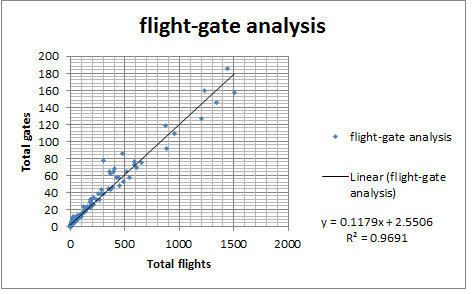
\includegraphics[width=0.8\textwidth]{img-gate-flight-nodelay.png}
    \caption{Relationship between the number of flights and the number of gates when there is no delay}
    \label{fig:gate-flight-nodelay}
\end{figure}

\subsubsection{Gate Collisions} We do two experiments in this part. We add random delay to the first experiments while we use the actual delays from the dataset in the second experiments. After adding delays, we add the number of gate collisions. Gate collisions only occur when there is an overlapping between two consecutive intervals of any gate.
\paragraph{Random delays} Figure~\ref{fig:flight-delay-distribution} shows that the highest probability density is around 0. In other words, most of the time, there are no delays in flights. The density function drops drastically as the delay grows larger. This distribution is one of long-tailed distributions, which have a large number of occurrences around the central part of the distribution. We tried several distribution functions and found that Weibull distribution with $\lambda = 0.7$ and $k = 20$ models the flight delay very well as shown in Figure~\ref{fig:flight-delay-model}. Therefore, we add delays based on this distribution to the result we have found earlier to find the number of gate collisions. Hence, if there is a delay, $d$, in the flight and the original interval is $[s_i, j_i)$, the updated interval will be $[s_i, j_i+d)$. \par
\begin{figure}
    \centering
    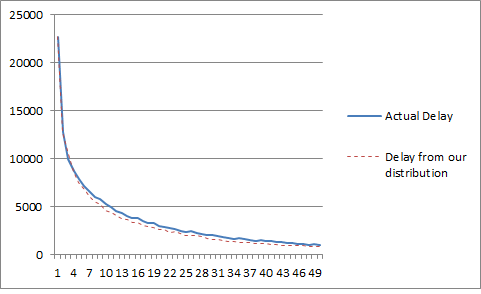
\includegraphics[width=0.8\textwidth]{img-flight-delay-distribution.png}
    \caption{Comparison between the real delay and our estimated delay}
    \label{fig:flight-delay-distribution}
\end{figure}
The result of the experiment is shown in Figure~\ref{fig:flight-collision-random}. The number of gate collisions can be estimated as a linear function with the number of flights, $y = 03.693x-7.3281$, where $y$ is the number of gate collisions and $x$ is the number of flights. \par
\begin{figure}
    \centering
    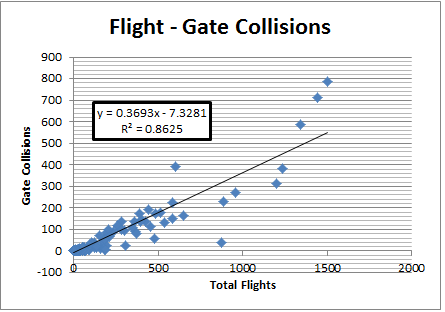
\includegraphics[width=0.8\textwidth]{img-flight-collision-random.png}
    \caption{Relationship between the number of gate collisions and the number of flights with random delay}
    \label{fig:gate-flight-collision-random}
\end{figure}
\paragraph{Actual delays} Another experiment is run on the actual taking-off time of each flight. In the date set, there are some flights taking off earlier than scheduling. However, our problem focuses on the effect of delay. Hence, we ignore that information. The result of the experiment is shown in Figure~\ref{fig:flight-collision}. The number of gate collisions of the actual data is fewer than that with random delays and can be estimated as $y = 0.2502x-5.3475$. \par
\begin{figure}
    \centering
    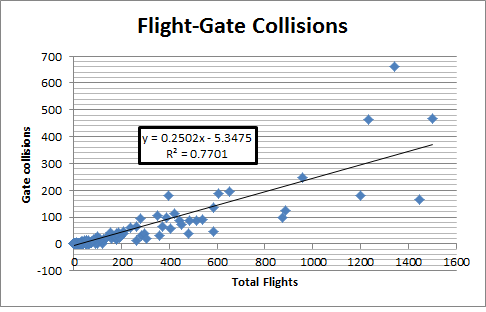
\includegraphics[width=0.8\textwidth]{img-flight-collision.png}
    \caption{Relationship between the number of gate collisions and the number of flights with actual delay}
    \label{fig:gate-flight-collision}
\end{figure}

\subsubsection{Overflow gates}
In this section, we use the first day of January data for all the airport. We run three algorithms to handle the delays: the optimal Algorithm~\ref{algo:p3-opt}, our Algorithm~\ref{algo:p3}, and the one that runs Algorithm~\ref{algo:p2} on all the collided flights and the results are shown in Figure~\ref{fig:overflow}. It is shown that our proposed Algorithm~\ref{algo:p3} has similar performance to the optimal solution. It is more suitable to use this algorithm when rescheduling is expensive.
\begin{figure}
    \centering
    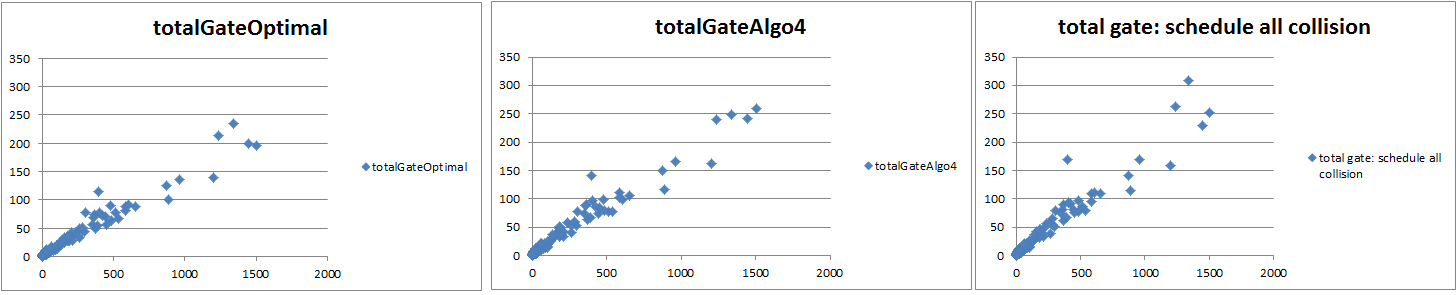
\includegraphics[width=1.2\textwidth]{img-overflow.png}
    \caption{The left figure shows the relationship between the number of optimal gates given a list of flights with actual delay. The middle figure shows the number of gates from Algorith~\ref{algo:p3}. The right most figure shows the result from the algorithm that schedules all gate collisions.}
    \label{fig:overflow}
\end{figure}

\section{Conclusions and Future Work}
\label{sec:conc}

\bibliographystyle{unsrt}
\bibliography{ref}

\section*{Appendix}
\subsection*{SQL Queries for Dataset Analysis}
\begin{enumerate}
\item Find airports with top 5 highest number of outgoing flights
\begin{lstlisting}[frame=single, language=SQL]
SELECT origin_airport_id\
	, COUNT(*) as origin_total_flights
FROM flight
GROUP BY origin_airport_id
ORDER BY origin_total_flights DESC ;
\end{lstlisting}
\item Find airports with top 5 highest number of incoming flights
\begin{lstlisting}[frame=single, language=SQL]
SELECT dest_airport_id
	, COUNT(*) as dest_total_flights
FROM flight
GROUP BY dest_airport_id
ORDER BY dest_total_flights DESC ;
\end{lstlisting}
\item Find the total number of delays

\begin{lstlisting}[frame=single, language=SQL]
SELECT fl_date, fl_month, fl_year
	, COUNT(*) as total_delay
FROM flight
WHERE cancelled = 0 AND dep_delay > 0
GROUP BY fl_date, fl_month, fl_year
ORDER BY total_delay DESC;
\end{lstlisting}
\item Find the average delay of DFW airport of each day.
\begin{lstlisting}[frame=single, language=SQL]
SELECT f1.fl_date, f1.fl_month, f1.fl_year
	, 1.0*f2.total_delay/f1.total_flight 
	as percentage
FROM
	(SELECT fl_date, fl_month, fl_year
	, COUNT(*) as total_flight
	FROM flight
	WHERE origin_airport_id = 11298
	GROUP BY fl_date, fl_month, fl_year) f1,
	(SELECT fl_date, fl_month, fl_year
	, SUM(dep_delay) as total_delay
	FROM flight
	WHERE origin_airport_id = 11298
		AND cancelled = 0
		AND dep_delay > 0
	GROUP BY fl_date, fl_month, fl_year ) f2
WHERE f1.fl_date = f2.fl_date
	AND f1.fl_month = f2.fl_month
	AND f1.fl_year = f2.fl_year
ORDER BY percentage DESC
LIMIT 10;
\end{lstlisting}
\end{enumerate}

\end{document}